\documentclass[11pt,a4paper]{article}

\usepackage[utf8]{inputenc}
\usepackage[T1]{fontenc}
\usepackage[spanish,es-nodecimaldot]{babel}
\usepackage{lmodern}
\usepackage{microtype}
\usepackage{geometry}
\geometry{top=2.2cm,bottom=2.3cm,left=2.2cm,right=2.2cm}
\usepackage{graphicx}
\graphicspath{{../results/figures_f2/}}
\usepackage{booktabs}
\usepackage{tabularx}
\usepackage{array}
\usepackage{longtable}
\usepackage{multirow}
\usepackage{float}
\usepackage{caption}
\usepackage{subcaption}
\usepackage{enumitem}
\usepackage{xcolor}
\usepackage{hyperref}
\usepackage{fancyhdr}
\usepackage[most]{tcolorbox}
\usepackage{amsmath}
\usepackage{siunitx}
\usepackage{titlesec}

\definecolor{unabblue}{HTML}{1F4E79}
\definecolor{lightgray}{HTML}{F4F4F4}
\definecolor{darkgray}{HTML}{4A4A4A}
\hypersetup{
  colorlinks=true,
  linkcolor=unabblue,
  urlcolor=unabblue,
  citecolor=unabblue,
  pdftitle={Evaluación Formativa 2 - Modelamiento Predictivo WeatherAUS},
  pdfauthor={Enzo Pinilla, Claudio Alarcón y Luis Rodrigo Espinoza}
}

\pagestyle{fancy}
\fancyhf{}
\fancyfoot[L]{\footnotesize Magíster en Ciencia de Datos e Inteligencia Artificial}
\fancyfoot[R]{\footnotesize \thepage}
\renewcommand{\headrulewidth}{0pt}
\renewcommand{\footrulewidth}{0.4pt}

\titleformat{\section}{\Large\bfseries}{\thesection}{0.7em}{}
\titleformat{\subsection}{\large\bfseries}{\thesubsection}{0.7em}{}
\setlist[itemize]{leftmargin=1.2em,itemsep=0.25em,topsep=0.35em}
\setlist[enumerate]{leftmargin=1.5em,itemsep=0.25em,topsep=0.35em}
\captionsetup{font=small,labelfont=bf}
\sisetup{output-decimal-marker={,}}

\newcolumntype{Y}{>{\raggedright\arraybackslash}X}
\newcolumntype{C}[1]{>{\centering\arraybackslash}p{#1}}
\newcolumntype{R}[1]{>{\raggedleft\arraybackslash}p{#1}}

\begin{document}

\begin{titlepage}
\thispagestyle{empty}
\begin{center}

\includegraphics[width=0.28\textwidth]{logo_unab.png}\par
\vspace{0.9cm}
{\large\bfseries MAGÍSTER EN CIENCIA DE DATOS E INTELIGENCIA ARTIFICIAL}\par
\vspace{0.25cm}
{\large MCDI501: Estadística Computacional para la Toma de Decisiones}\par
\vspace{1.2cm}
{\LARGE\bfseries Evaluación Formativa 2}\par
\vspace{0.25cm}
{\Large Práctica de Modelamiento Predictivo}\par
\vspace{1.1cm}
{\large Informe de práctica grupal · sin ponderación (formativa)}\par
\vspace{1.6cm}
\begin{tabular}{>{\bfseries}p{4.2cm}p{10cm}}
Título del proyecto: & Predicción de lluvia del día siguiente en Australia \\
Integrantes: & Enzo Pinilla, Claudio Alarcón y Luis Rodrigo Espinoza \\
Dataset: & WeatherAUS / Rain in Australia \\
Docente: & Dr. Jean Paul Maidana González \\
Fecha: & 10 de julio de 2026 \\
Repositorio GitHub: & \href{https://github.com/sauriomac/mcdi501-estadistica-computacional-grupo2}{mcdi501-estadistica-computacional-grupo2} \\
\end{tabular}
\vfill
\end{center}
\end{titlepage}

\pagenumbering{arabic}
\setcounter{page}{1}

\subsection*{Conexión con evaluaciones anteriores}
Esta práctica reutiliza los hallazgos de S1 y su validación en S2 para construir una primera línea base de clasificación. El objetivo no es redescubrir el conjunto de datos, sino convertir la evidencia previa en decisiones explícitas de selección de variables, tratamiento de faltantes, manejo de colas pesadas y evaluación de un modelo logístico. La variable objetivo es \texttt{RainTomorrow}, codificada como 1 cuando llueve al día siguiente y 0 en caso contrario.

\tableofcontents
\newpage

\section{Preparación de datos para el modelamiento}

\subsection{Referencia a los hallazgos de S1 y S2}
El conjunto WeatherAUS contiene observaciones meteorológicas diarias de estaciones australianas. Para el modelamiento se utilizaron 142.193 registros con objetivo válido. La clase positiva \texttt{RainTomorrow=Yes} representa 22,42\% de los casos, por lo que existe un desbalance moderado que obliga a interpretar accuracy junto con precision, recall y F1-score.

S1 identificó asociaciones relevantes entre el objetivo y \texttt{Humidity3pm}, \texttt{RainToday}, \texttt{Humidity9am}, \texttt{Pressure9am}, \texttt{Rainfall} y \texttt{WindGustSpeed}. También documentó una correlación cercana a 0,985 entre \texttt{MaxTemp} y \texttt{Temp3pm}, por lo que no resulta conveniente emplearlas simultáneamente sin un control explícito de multicolinealidad. Además, \texttt{Sunshine} y \texttt{Evaporation} presentan aproximadamente 48\% y 43\% de datos faltantes, respectivamente, mientras que \texttt{Rainfall} y \texttt{WindGustSpeed} exhiben colas derechas y valores extremos.

S2 validó mediante bootstrap que las correlaciones de \texttt{Humidity3pm}, \texttt{RainToday\_bin}, \texttt{Humidity9am}, \texttt{Pressure9am} y \texttt{Rainfall} conservaron su signo y que sus intervalos de confianza al 95\% no incluyeron cero. También mostró que aplicar la regla IQR a \texttt{Rainfall} marca cerca de 18\% de las observaciones, principalmente por su concentración de ceros y cola pesada; por ello no se eliminaron automáticamente como errores, sino que se aplicó la transformación \(\log(1+x)\).

\begin{table}[H]
\centering
\caption{Correlaciones de S2 utilizadas para fundamentar la selección.}
\small
\begin{tabular}{lrrrr}
\toprule
Variable & $r$ observado & IC95 inf. & IC95 sup. & Conclusión \\
\midrule
Humidity3pm   &  0,4462 &  0,4418 &  0,4505 & Estable \\
RainToday\_bin & 0,3131 &  0,3074 &  0,3189 & Estable \\
Humidity9am   &  0,2572 &  0,2526 &  0,2616 & Estable \\
Pressure9am   & -0,2464 & -0,2516 & -0,2411 & Estable \\
Rainfall      &  0,2390 &  0,2319 &  0,2462 & Estable \\
\bottomrule
\end{tabular}
\end{table}

\subsection{Selección de variables y tratamiento aplicado}
Se seleccionaron cinco predictores. \texttt{Humidity3pm} representa la señal de mayor asociación estable; \texttt{RainToday\_bin} incorpora la ocurrencia reciente de lluvia; \texttt{Pressure9am} aporta una asociación negativa; \texttt{Rainfall\_log1p} mantiene la información de precipitación controlando la cola pesada; y \texttt{WindGustSpeed} agrega una dimensión física distinta de humedad, presión y lluvia. \texttt{Humidity9am} se reservó para S3 para limitar el modelo a cinco variables y evitar duplicar en exceso la información de humedad.

\begin{table}[H]
\centering
\caption{Valores faltantes en los predictores antes de la imputación.}
\small
\begin{tabular}{lrr}
\toprule
Variable & Faltantes & Porcentaje \\
\midrule
Pressure9am      & 14.014 & 9,8556\% \\
WindGustSpeed    & 9.270  & 6,5193\% \\
Humidity3pm      & 3.610  & 2,5388\% \\
RainToday\_bin  & 1.406  & 0,9888\% \\
Rainfall\_log1p & 1.406  & 0,9888\% \\
\bottomrule
\end{tabular}
\end{table}

La imputación se realizó con la mediana para las variables continuas, por su robustez frente a asimetría y extremos, y con la moda para \texttt{RainToday\_bin}. Los parámetros de imputación y estandarización se estimaron exclusivamente sobre entrenamiento, evitando fuga de información. Las variables continuas se estandarizaron; la variable binaria se conservó en escala 0/1.

\begin{figure}[H]
\centering
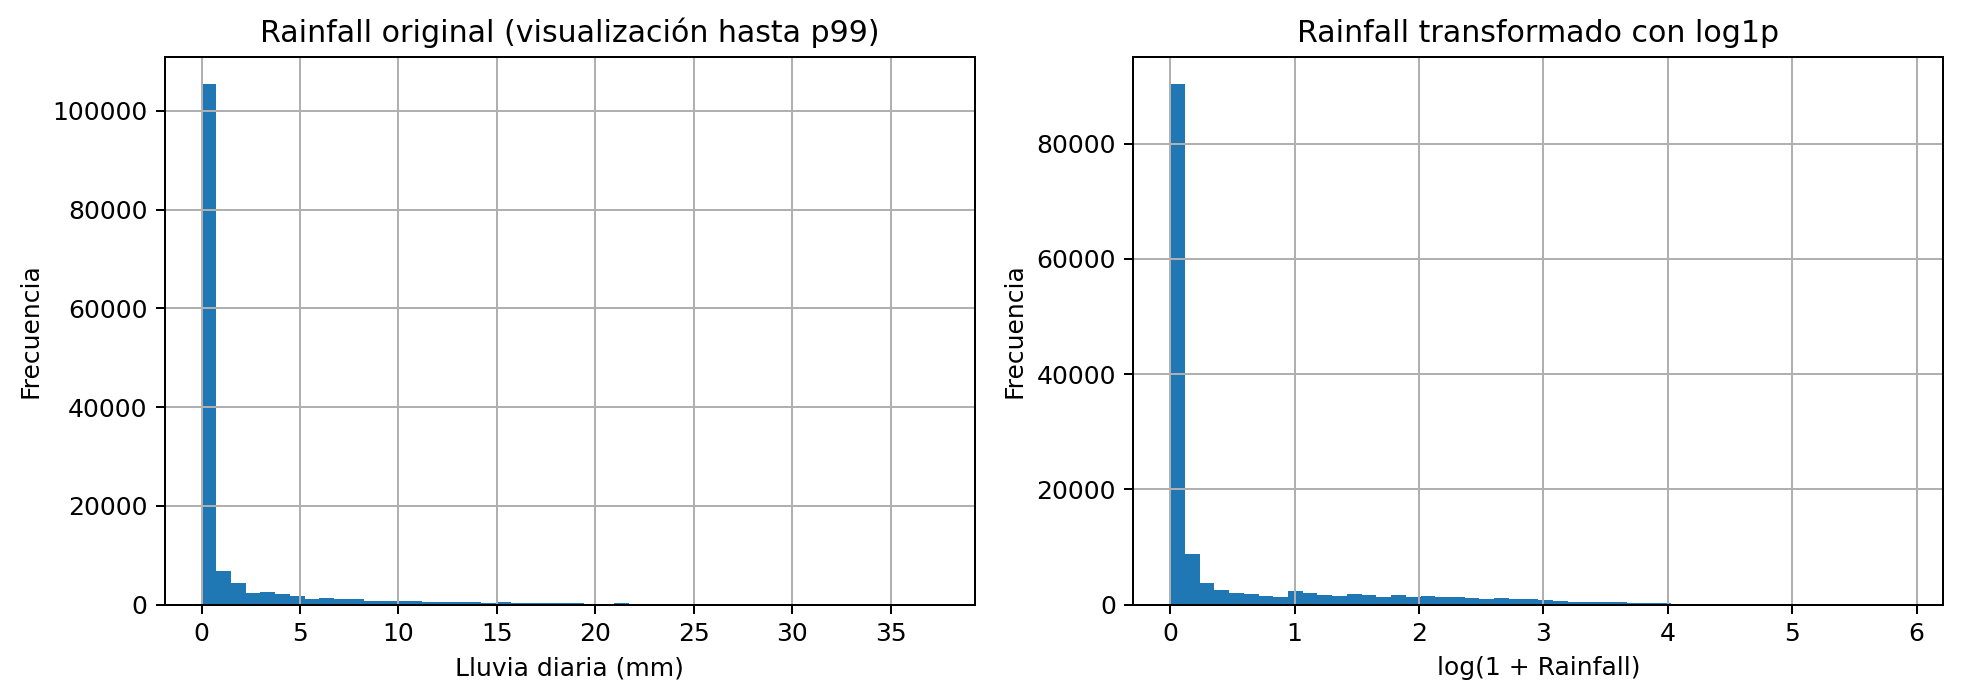
\includegraphics[width=0.90\textwidth]{rainfall_transform.png}
\caption{Distribución de \texttt{Rainfall} antes y después de la transformación \(\log(1+x)\). La transformación reduce la dominancia visual de la cola sin eliminar eventos reales de lluvia.}
\end{figure}

La partición se realizó en 70\% para entrenamiento y 30\% para prueba, estratificando por la variable objetivo. El conjunto de entrenamiento quedó con 99.535 observaciones y el de prueba con 42.658; ambos conservaron una proporción positiva de 0,2242.

\begin{table}[H]
\centering
\caption{Parámetros de imputación aprendidos exclusivamente en entrenamiento.}
\small
\begin{tabular}{lrl}
\toprule
Variable & Valor aprendido & Estrategia \\
\midrule
Humidity3pm      & 52,0   & Mediana \\
Pressure9am      & 1.017,6 & Mediana \\
Rainfall\_log1p & 0,0    & Mediana \\
WindGustSpeed    & 39,0   & Mediana \\
RainToday\_bin  & 0,0    & Moda \\
\bottomrule
\end{tabular}
\end{table}

\begin{figure}[H]
\centering
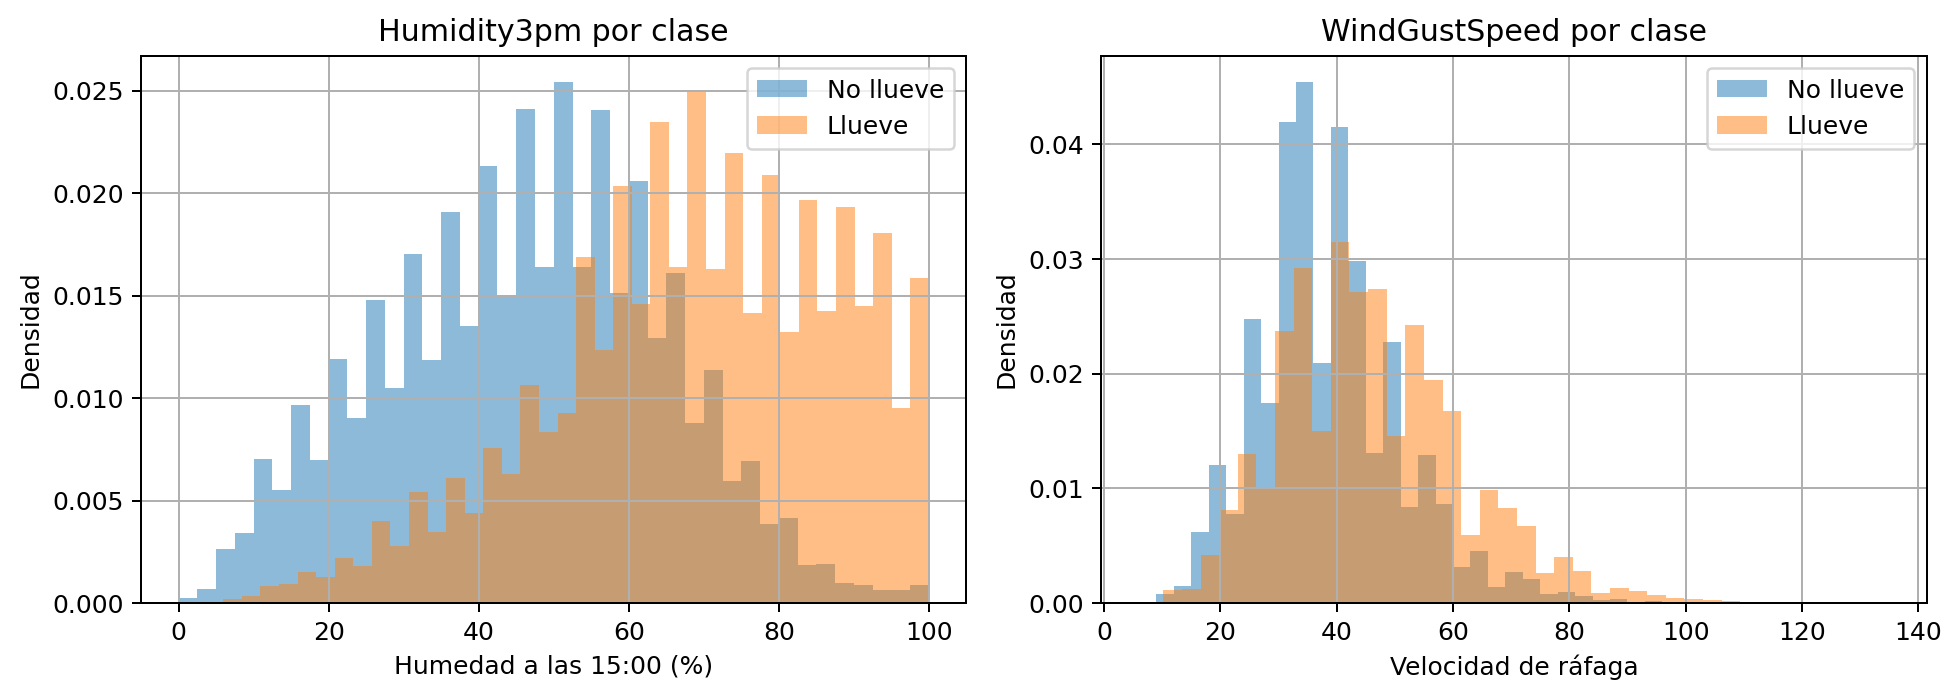
\includegraphics[width=0.92\textwidth]{predictor_distributions.png}
\caption{Distribución de dos predictores por clase. La humedad de la tarde y la velocidad de ráfaga muestran desplazamientos hacia valores mayores en los días con lluvia posterior.}
\end{figure}

\section{Modelo de regresión logística}

\subsection{Ajuste e interpretación de coeficientes}
El modelo se ajustó mediante \texttt{statsmodels.Logit} sobre los datos de entrenamiento procesados. Convergió correctamente con 99.535 observaciones, cinco predictores y un pseudo \(R^2\) de McFadden de 0,2793. Para los predictores continuos estandarizados, cada odds ratio representa el cambio multiplicativo en las odds de lluvia ante un aumento de una desviación estándar. En \texttt{RainToday\_bin}, el odds ratio compara un día con lluvia frente a uno sin lluvia, manteniendo constantes las demás variables.

\begin{table}[H]
\centering
\caption{Coeficientes, odds ratios e intervalos de confianza del modelo logístico.}
\scriptsize
\begin{tabular}{lrrrrrr}
\toprule
Variable & Coef. & EE & $z$ & $p$ & OR & IC95 OR \\
\midrule
Constante          & -1,7666 & 0,0142 & -124,2102 & $<0,001$ & 0,1709 & [0,1662; 0,1757] \\
Humidity3pm        &  1,2510 & 0,0116 &  107,8924 & $<0,001$ & 3,4940 & [3,4154; 3,5743] \\
RainToday\_bin    &  0,1204 & 0,0390 &    3,0870 & 0,002 & 1,1280 & [1,0449; 1,2176] \\
Pressure9am        & -0,3856 & 0,0101 &  -38,0081 & $<0,001$ & 0,6800 & [0,6666; 0,6937] \\
Rainfall\_log1p   &  0,2159 & 0,0163 &   13,2479 & $<0,001$ & 1,2409 & [1,2019; 1,2812] \\
WindGustSpeed      &  0,4479 & 0,0097 &   46,0834 & $<0,001$ & 1,5650 & [1,5354; 1,5951] \\
\bottomrule
\end{tabular}
\end{table}

\texttt{Humidity3pm} es el predictor dominante: una desviación estándar adicional multiplica las odds de lluvia por aproximadamente 3,49. \texttt{WindGustSpeed} presenta un odds ratio de 1,57, de modo que ráfagas más intensas se relacionan con mayor probabilidad relativa de lluvia. \texttt{Rainfall\_log1p} tiene un odds ratio de 1,24 y \texttt{RainToday\_bin} uno de 1,13, ambos coherentes con la persistencia de condiciones lluviosas. \texttt{Pressure9am} actúa como factor protector: una desviación estándar adicional reduce las odds estimadas en alrededor de 32\%. Todos los predictores fueron estadísticamente significativos al 5\%.

La significancia no equivale por sí sola a utilidad predictiva. La magnitud de los efectos, sus intervalos y el desempeño en el conjunto de prueba deben analizarse conjuntamente.

\subsection{Diagnóstico de multicolinealidad}
El factor de inflación de la varianza (VIF) se calculó sobre los predictores procesados. Como referencia práctica, valores superiores a 5 requieren revisión y valores sobre 10 suelen indicar un problema grave.

\begin{table}[H]
\centering
\caption{Diagnóstico VIF de los predictores.}
\small
\begin{tabular}{lr}
\toprule
Variable & VIF \\
\midrule
Rainfall\_log1p & 2,708 \\
RainToday\_bin  & 2,513 \\
Pressure9am     & 1,253 \\
WindGustSpeed   & 1,241 \\
Humidity3pm     & 1,194 \\
\bottomrule
\end{tabular}
\end{table}

El VIF máximo fue 2,708, por lo que no se observa multicolinealidad problemática. Este resultado es coherente con la decisión de no incorporar simultáneamente \texttt{MaxTemp} y \texttt{Temp3pm}.

\begin{figure}[H]
\centering
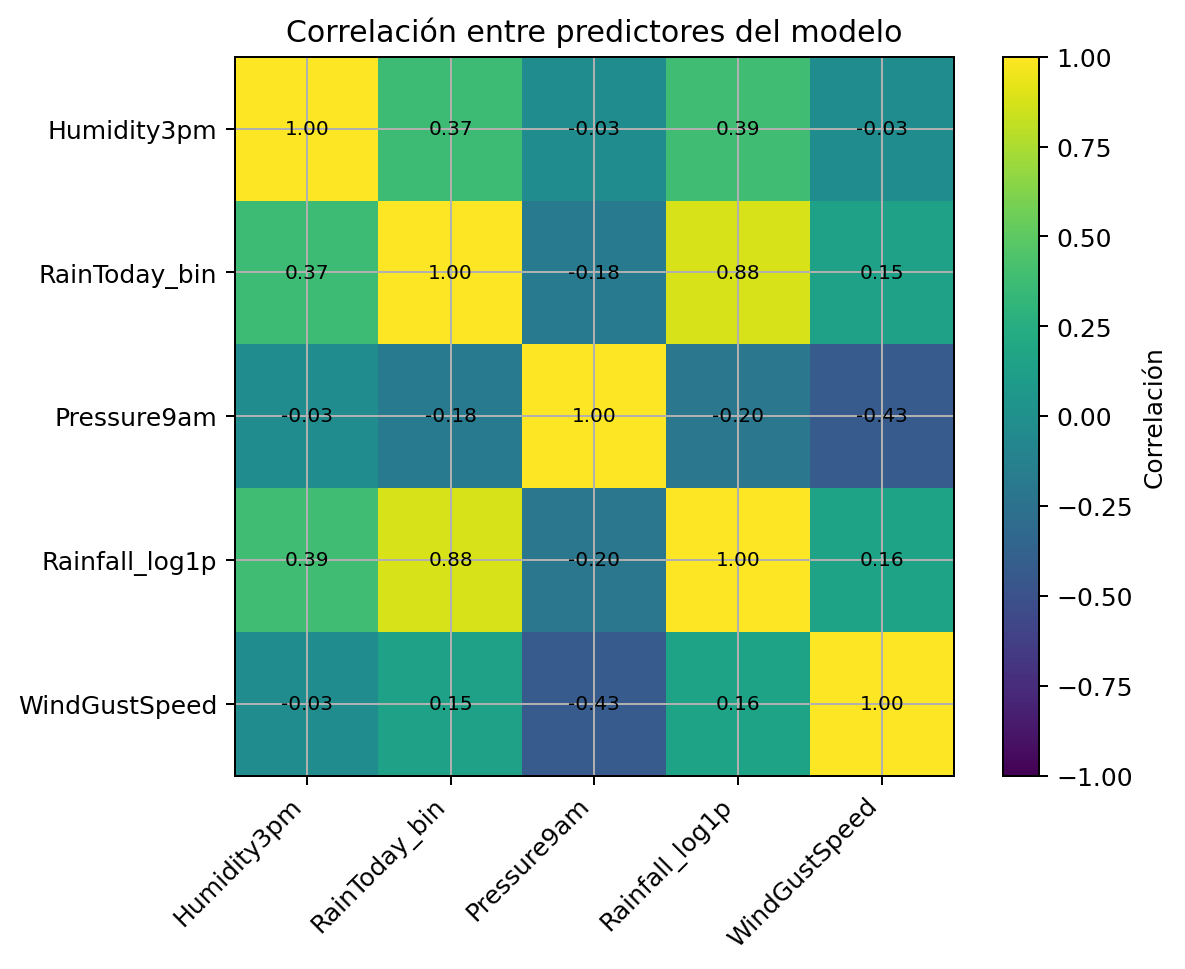
\includegraphics[width=0.70\textwidth]{predictor_correlation.png}
\caption{Matriz de correlaciones de los predictores procesados. No se observan asociaciones lineales suficientemente altas como para comprometer la estabilidad del ajuste.}
\end{figure}

\section{Evaluación de desempeño predictivo}

\subsection{Matriz de confusión y métricas}
Las probabilidades se calcularon sobre el conjunto de prueba y se transformaron en clases mediante el umbral convencional de 0,5. La matriz de confusión produjo 31.401 verdaderos negativos, 1.694 falsos positivos, 5.182 falsos negativos y 4.381 verdaderos positivos.

\begin{figure}[H]
\centering
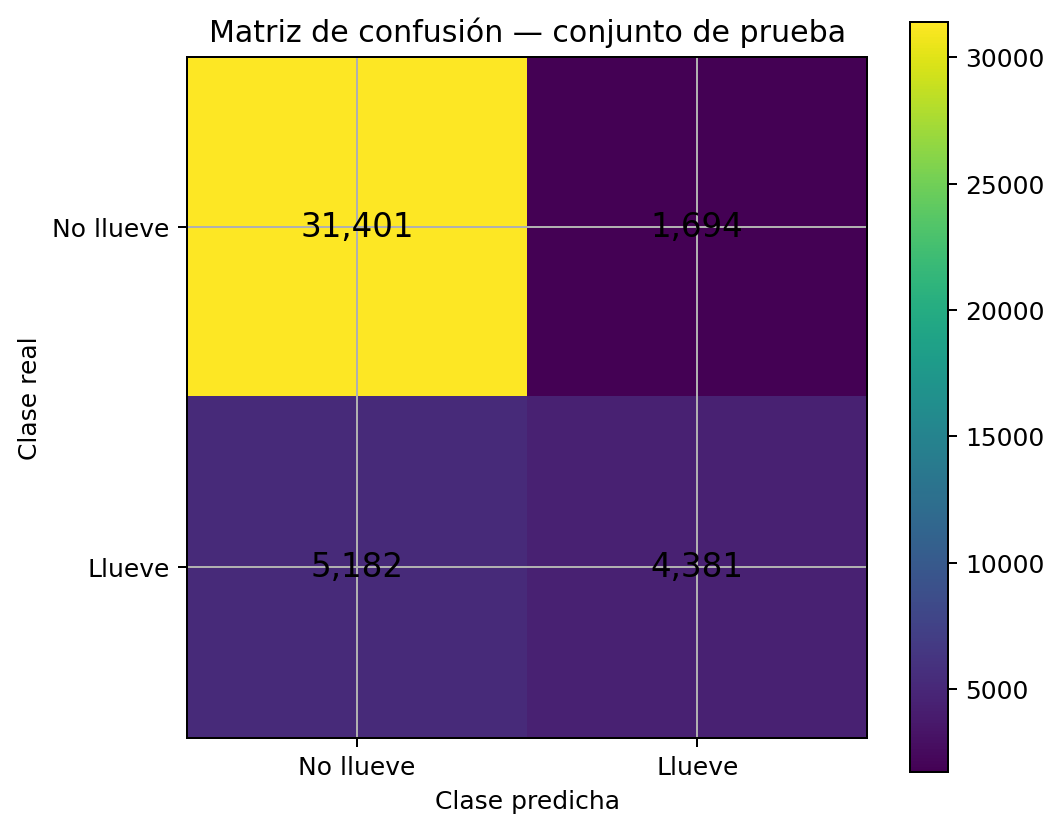
\includegraphics[width=0.62\textwidth]{confusion_matrix.png}
\caption{Matriz de confusión sobre el conjunto de prueba con umbral 0,5.}
\end{figure}

\begin{table}[H]
\centering
\caption{Métricas de desempeño en el conjunto de prueba.}
\small
\begin{tabular}{lr}
\toprule
Métrica & Valor \\
\midrule
Accuracy & 0,8388 \\
Precision & 0,7212 \\
Recall / sensibilidad & 0,4581 \\
F1-score & 0,5603 \\
Especificidad & 0,9488 \\
Balanced accuracy & 0,7035 \\
ROC-AUC & 0,8415 \\
PR-AUC & 0,6623 \\
Accuracy de la clase mayoritaria & 0,7758 \\
\bottomrule
\end{tabular}
\end{table}

La accuracy de 83,88\% supera el 77,58\% de un clasificador trivial que siempre pronostica ``no llueve''. La precision de 72,12\% indica que, cuando el modelo anuncia lluvia, acierta en algo más de siete de cada diez casos. Sin embargo, el recall de 45,81\% muestra la principal limitación: el modelo detecta menos de la mitad de los días que efectivamente tendrán lluvia. El F1-score de 0,5603 resume el desequilibrio entre una precision razonable y una sensibilidad todavía moderada.

En un escenario donde omitir lluvia tenga un costo operacional elevado, no sería suficiente mantener el umbral 0,5. El ajuste del punto de corte o la ponderación de la clase positiva deberían priorizarse en S3.

\subsection{Curva ROC y AUC}
La curva ROC resume la relación entre sensibilidad y tasa de falsos positivos a través de todos los umbrales. El ROC-AUC obtenido fue 0,8415, valor que se interpreta como una capacidad de discriminación buena. En términos probabilísticos, el modelo asigna una puntuación mayor a un día lluvioso que a uno no lluvioso en aproximadamente 84\% de los pares tomados al azar.

\begin{figure}[H]
\centering
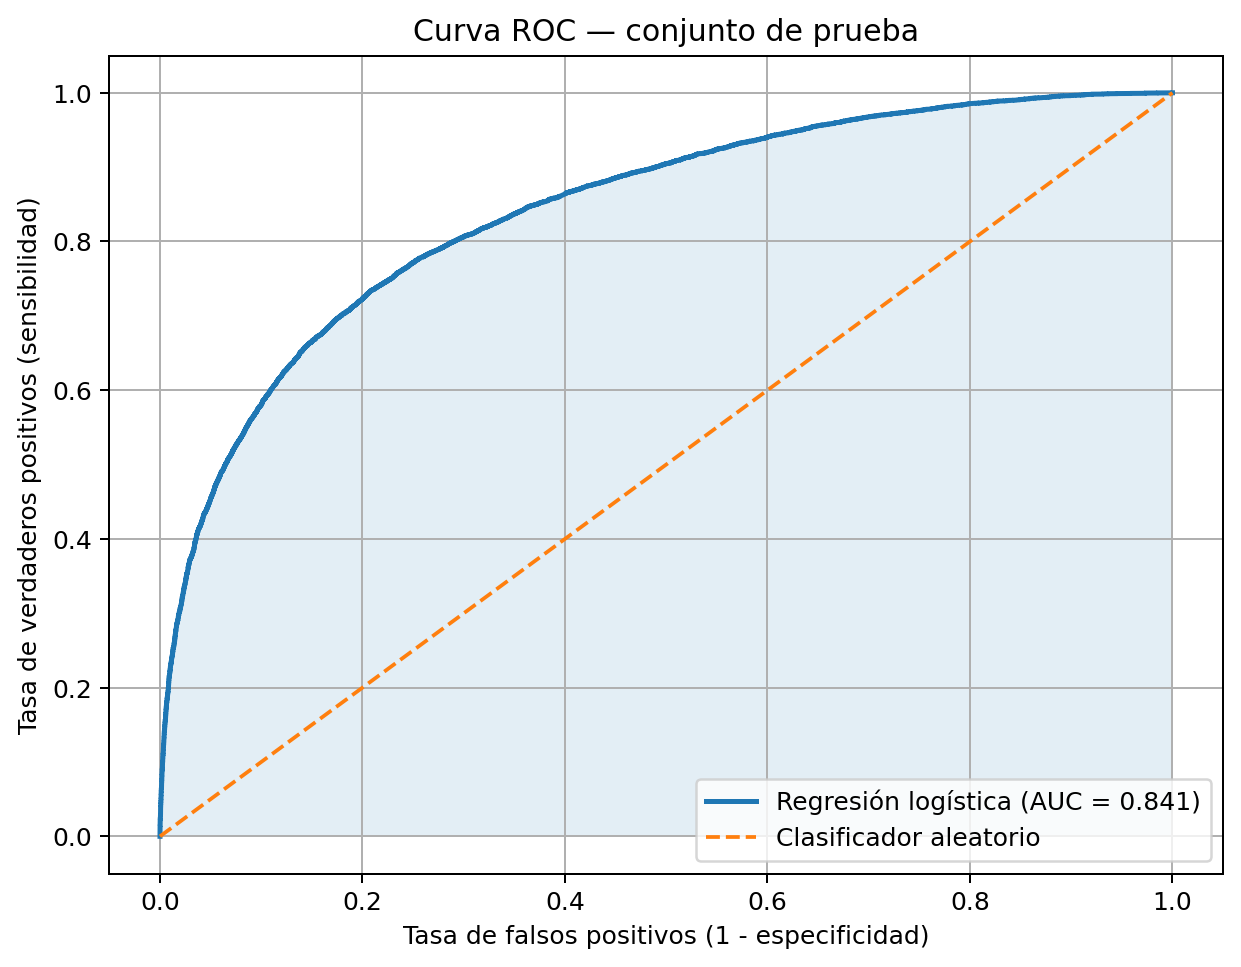
\includegraphics[width=0.72\textwidth]{roc_curve.png}
\caption{Curva ROC del modelo logístico sobre el conjunto de prueba. El AUC de 0,8415 evidencia una separación útil entre las clases.}
\end{figure}

El buen AUC no contradice el recall moderado observado con umbral 0,5: el modelo ordena adecuadamente el riesgo, pero el punto de corte actual es conservador para declarar lluvia. Como métrica complementaria ante el desbalance, el PR-AUC fue 0,6623.

\section{Síntesis y reflexión}
La Formativa 2 integró los resultados acumulados de S1 y S2 en un primer modelo predictivo reproducible. Desde S1 se heredaron la definición de \texttt{RainTomorrow} como objetivo binario, el desbalance de aproximadamente 22,4\%, el patrón de valores faltantes, la colinealidad extrema entre \texttt{MaxTemp} y \texttt{Temp3pm}, y el carácter asimétrico de \texttt{Rainfall} y \texttt{WindGustSpeed}. Estas observaciones evitaron seleccionar variables solo por disponibilidad: se excluyeron \texttt{Sunshine} y \texttt{Evaporation} por su alta ausencia, no se combinaron temperaturas casi duplicadas y se transformó \texttt{Rainfall} con \(\log(1+x)\) en lugar de eliminar como ``outliers'' numerosos días con lluvia real.

S2 aportó validación metodológica. Las correlaciones de \texttt{Humidity3pm}, \texttt{RainToday\_bin}, \texttt{Pressure9am} y \texttt{Rainfall} mantuvieron su signo en 10.000 remuestras bootstrap, mientras que los parámetros de \texttt{Humidity3pm}, \texttt{WindGustSpeed} y la proporción de lluvia fueron consistentes entre métodos clásicos y de remuestreo. Con esa evidencia se seleccionaron cinco predictores: humedad de la tarde, lluvia actual, presión matinal, lluvia transformada y velocidad de ráfaga. La imputación se realizó con mediana para continuas y moda para la binaria, ajustando todo únicamente en entrenamiento. La partición 70/30 fue estratificada y las variables continuas se estandarizaron.

El modelo logístico fue estadísticamente coherente: todos los predictores resultaron significativos y los VIF permanecieron bajo 3, sin evidencia de multicolinealidad problemática. \texttt{Humidity3pm} fue la señal dominante, mientras que \texttt{Pressure9am} mostró un efecto protector. En prueba, el modelo obtuvo accuracy de 83,9\%, precision de 72,1\%, recall de 45,8\%, F1 de 0,56 y ROC-AUC de 0,841. El AUC evidencia buena capacidad de discriminación; no obstante, el umbral 0,5 deja sin detectar más de la mitad de los días lluviosos, por lo que la evaluación no puede basarse únicamente en accuracy.

De cara a S3, las mejoras prioritarias son comparar imputación simple con alternativas más informativas, ajustar o validar el umbral según el costo de falsos negativos, incorporar ponderación de clases, reportar PR-AUC, evaluar regularización y posibles interacciones o no linealidades, y validar la estabilidad de los coeficientes mediante bootstrap. Además, una partición temporal o agrupada por \texttt{Location} sería más realista que una división aleatoria, porque las observaciones de una misma estación y fechas cercanas no son completamente independientes. Esta formativa deja una línea base interpretable sobre la cual comparar modelos más completos sin perder coherencia con S1 y S2.

\clearpage
\section{Bibliografía}
\begin{thebibliography}{9}
\bibitem{efron1993} Efron, B., \& Tibshirani, R. J. (1993). \textit{An Introduction to the Bootstrap}. Chapman \& Hall/CRC.
\bibitem{hosmer2013} Hosmer, D. W., Lemeshow, S., \& Sturdivant, R. X. (2013). \textit{Applied Logistic Regression} (3.\textsuperscript{a} ed.). Wiley.
\bibitem{james2013} James, G., Witten, D., Hastie, T., \& Tibshirani, R. (2013). \textit{An Introduction to Statistical Learning}. Springer.
\bibitem{kaggle2017} Kaggle. (2017). \textit{Rain in Australia / WeatherAUS} [Conjunto de datos].
\bibitem{maidana2026} Maidana González, J. P. (2026). Materiales del curso MCDI501. Universidad Andrés Bello.
\bibitem{pedregosa2011} Pedregosa, F., et al. (2011). Scikit-learn: Machine Learning in Python. \textit{Journal of Machine Learning Research, 12}, 2825--2830.
\bibitem{seabold2010} Seabold, S., \& Perktold, J. (2010). Statsmodels: Econometric and Statistical Modeling with Python. \textit{Proceedings of the 9th Python in Science Conference}, 92--96.
\end{thebibliography}

\end{document}
